%%%%%%%%%%%%%%%%%%%%%%%%%%%%%%%%%%%%%%%%%%%%%%%%%%%%%%%
%                   File: OSAmeetings.tex             %
%                  Date: 20 September 2021            %
%                                                     %
%     For preparing LaTeX manuscripts for submission  %
%       submission to Optica meetings and conferences %
%                                                     %
%       (c) 2021 Optica                               %
%%%%%%%%%%%%%%%%%%%%%%%%%%%%%%%%%%%%%%%%%%%%%%%%%%%%%%%

\documentclass[letterpaper,10pt]{article} 
%% if A4 paper needed, change letterpaper to A4

\usepackage{osameet3} %% use version 3 for proper copyright statement

%% standard packages and arguments should be modified as needed
\usepackage{amsmath,amssymb}
\usepackage[colorlinks=true,bookmarks=false,citecolor=blue,urlcolor=blue]{hyperref} %pdflatex
%\usepackage[breaklinks,colorlinks=true,bookmarks=false,citecolor=blue,urlcolor=blue]{hyperref} %latex w/dvipdf
\usepackage[english]{babel}
\newtheorem{theorem}{Theorem}
\newtheorem{corollary}{Corollary}
\newtheorem{lemma}[theorem]{Lemma}
\newtheorem{conjecture}{Conjecture}
\newtheorem{definition}{Definition}
\newtheorem{workdefinition}{Working Definition}
\newtheorem{problem}{Problem}

\usepackage{color}
\newcommand\dashto{\mathrel{
  -\mkern-6mu{\to}\mkern-20mu{\color{white}\bullet}\mkern12mu
}}

\newcommand\indep{\perp \!\!\! \perp}

\usepackage{caption}
\usepackage{subcaption}

\usepackage{tikz} 



\begin{document}

\title{Mid-Semester Report: Cyclic Causality}

\author{David Reber}
\address{Columbia University}
\email{david.reber@columbia.edu}
%%Uncomment the following line to override copyright year from the default current year.
\copyrightyear{2022}


\begin{abstract}
abstract
\end{abstract}

%%%%%%%%%%%%%%%%%%%%%%%%%%%%%%%%%%%%%%%%%%%%%%%%%%%%%%%%%%%%%%%%%%%%%%%%%%%%%%%%%%%%%%%

\section{Lit. Review: Foundations \cite{Foundations}}

`Foundations of structural causal models with cycles and latent variables' by Bongers et. al. \cite{Foundations} outlines a modeling framework for cyclic SCMs that is quite similar to Pearl's framework for acyclic SCMs.
Cycles are incorperated simply by allowing the function $F$ of the SCM $M=(U,V,F,P(U))$ to be dependent on any variables in $U\cup V$.
% While technically SCMs without a unique fixed point are can still be expressed within the framework, the authors focus primarily on situations where a unique fixed point exists.
This paper focuses on atomic interventions (which they call `perfect interventions').

Previously in the literature, it had already been established that many nice properties of acyclic SCMs can be lost once cycles are allowed. For example, 1. Potential response functions may not exist; 2. The observational / interventional / counterfactual distributions may not exist, or if they do, they may not be unique; 3. Marginalizing over variables may not be possible, or sensible; 4. d-separation may not hold (aka. the `directed global Markov property') 5. $\sigma$-separation may not hold (aka. the `general directed global Markov property'; a weaker form of d-separation); 6. the induced causal graph may not be consistent with the SCM's causal semantics. 

There are several aspects of this framework which contrast with Pearl \cite{pearl_2009}.
The authors emphasize almost-everywhere equivalence, with respect to the observational, interventional, and counterfactual distributions, or structural functions themselves. This empahsis implicitly impacts their definitions. For example, and notably, the definition of a variable's `parents' excludes any trivial dependancies: node $k$ is a parent of $i$ only if a measurable function cannot be found which does not depend on $k$ and almost-everywhere matches the structural function for node $i$. While this definition is semantically useful (we only say there's a parent if there's a dependence that really can't be ignored) it can be slightly confusing: for example, consider the two-node linear system of $x_1 = f_1(x_1,x_2)=0.5x_1+0.1x_2$ and $x_2 = f_2(x_1,x_2)=0.1x_1+0.5x_2$. According to the definitions of \cite{Foundations}, $x_1$ and $x_2$ are both parents of each other, yet no self-cycles exist, because there exists an SCM which is asymptotically equivalent without self-cycles. (This property of linear systems will be discussed further in Section \ref{section:learninglinear}; see Figure \ref{fig:SelfCycles}).

Besides presenting unifying notation and sythesizing a cohesive review of much of the work on cyclic SCMs, the authors also present their own significant contribution: simple SCMs. Simple SCMs are SCMs which are uniquely solvable with respect to every subset of variables. Intuitively, this means that every submodel has a unique fixed point (so the potential response function is well-defined for each submodel). This is a sufficient condition for the observational, interventional, and counterfactual distributions to exist and be unique. Furthermore, simple SCMs satisfy a weaker form of the d-sepearation criterion, called $\sigma$-separation (a.k.a. the general directed global Markov property). Simple SCMs are closed under marginalization, and the marginalization respects the latent projection (that is, the causal sematics of the causal diagram's subgraph match the structure of the submodel of the SCM).
The relationship of simple SCMs to previous classes of cyclic SCMs explored in the literature is shown in Figure \ref{fig:CylicClasses}. 
(For the sake of this review, it suffices to say that modular SCMs are a class of cyclic SCMs which contain the class of simple SCMs; causal constraint models, CCMs, are a generalization of SCMs which is expressive but lacks a satisfying graphical representation).
\begin{figure}
\centering
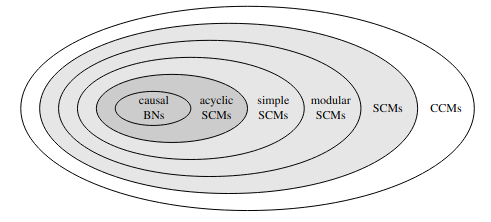
\includegraphics[width=.6\linewidth]{pics/cyclic_classes.png}
\caption{An inclusion diagram of various modeling frameworks for cyclic SCMs. Source\cite{Foundations}}
\label{fig:CylicClasses}
\end{figure}

% %%%%%%%%%%%%%%%%%%%%%%%%%%%%%%%%%%%%%%%%%%%%%%%%%%%%%%%%%%%%%%%%%%%%%%%%%%%%%%%%%%%%%%%

\section{Lit. Review: Learning Linear \cite{LearningLinear}} \label{section:learninglinear}
% \color{blue} In your own words, what are the most important aspects of the framework used in `Foundations'? \color{black}
% \begin{itemize}
%   \item 
% \end{itemize}

% \color{blue} In what ways does this framework differ from Pearl? Were there any surprises you encountered while reading? What confusions did you have that got cleared up? [TODO: cite Pearl]. \color{black}
% \begin{itemize}
%   \item 
% \end{itemize}

% \color{blue} What are the most significant results from `Foundations'? \color{black}
% \begin{itemize}
%   \item 
% \end{itemize}

% \color{blue} What sort of previous work is `Foundations' building on? \color{black}
% \begin{itemize}
%   \item 
% \end{itemize}

\begin{figure}
\centering
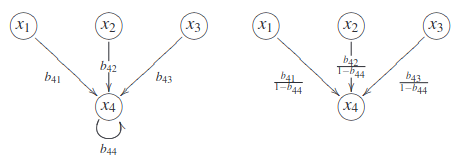
\includegraphics[width=.6\linewidth]{pics/self_cycles.png}
\caption{Source: \cite{LearningLinear}}
\label{fig:SelfCycles}
\end{figure}

% \color{red} TODO: \color{black}


% %%%%%%%%%%%%%%%%%%%%%%%%%%%%%%%%%%%%%%%%%%%%%%%%%%%%%%%%%%%%%%%%%%%%%%%%%%%%%%%%%%%%%%%

% \section{Lit. Review: Settable Systems \cite{White&Chalak}}
% \begin{itemize}
%   \item 
% \end{itemize}

% %%%%%%%%%%%%%%%%%%%%%%%%%%%%%%%%%%%%%%%%%%%%%%%%%%%%%%%%%%%%%%%%%%%%%%%%%%%%%%%%%%%%%%%

% \section{Lit. Review: Game Incomplete \cite{GameIncomplete}}
% \begin{itemize}
%   \item 
% \end{itemize}

% %%%%%%%%%%%%%%%%%%%%%%%%%%%%%%%%%%%%%%%%%%%%%%%%%%%%%%%%%%%%%%%%%%%%%%%%%%%%%%%%%%%%%%%

% \section{Lit. Review: Markov Properties \cite{MarkovCyclesLatent}}
% \begin{itemize}
%   \item 
% \end{itemize}

% %%%%%%%%%%%%%%%%%%%%%%%%%%%%%%%%%%%%%%%%%%%%%%%%%%%%%%%%%%%%%%%%%%%%%%%%%%%%%%%%%%%%%%%

% \section{Lit. Review: Dynamical Systems \cite{DynamicalSystems}}
% \begin{itemize}
%   \item 
% \end{itemize}

%%%%%%%%%%%%%%%%%%%%%%%%%%%%%%%%%%%%%%%%%%%%%%%%%%%%%%%%%%%%%%%%%%%%%%%%%%%%%%%%%%%%%%%

% pdflatex main
% bibtex main
% pdflatex main
% pdflatex main

\bibliographystyle{plain}
\bibliography{refs}

\end{document}
